
\documentclass[a4paper,12pt]{article}
\usepackage[latin1]{inputenc}
\usepackage[spanish,es-nodecimaldot]{babel}
\usepackage[T1]{fontenc}
\usepackage[intlimits]{amsmath}
\usepackage{graphicx}
\usepackage{a4wide}
\usepackage{float}

\graphicspath{{imagenes/}}

\title{\textsc{Modelo de Ising en 2D} \\ \vspace{2em} \Large{Introducci�n a la 
simulaci�n computacional}}
\author{\small{Luis Pizarro (lpizarro@cnea.gov.ar)} \\
        \small{Pablo Bellino (pbellino@gmail.com)}}

\date{Octubre de 2015}


\begin{document}
\maketitle

\begin{abstract}
Un resumen
\end{abstract}


\section{Introducci�n}
Empezamo

%\begin{eqnarray}
%  f_r(x) &=& \frac{4}{\pi - 4}\frac{x^2}{1+x^2} \\
%  f_\theta(x) &=& \frac{\sin(x)}{2} \\
%  f_\varphi(x) &=&  \frac{1}{2\pi} 
%\end{eqnarray}


\begin{figure}[H]
    \begin{center}
      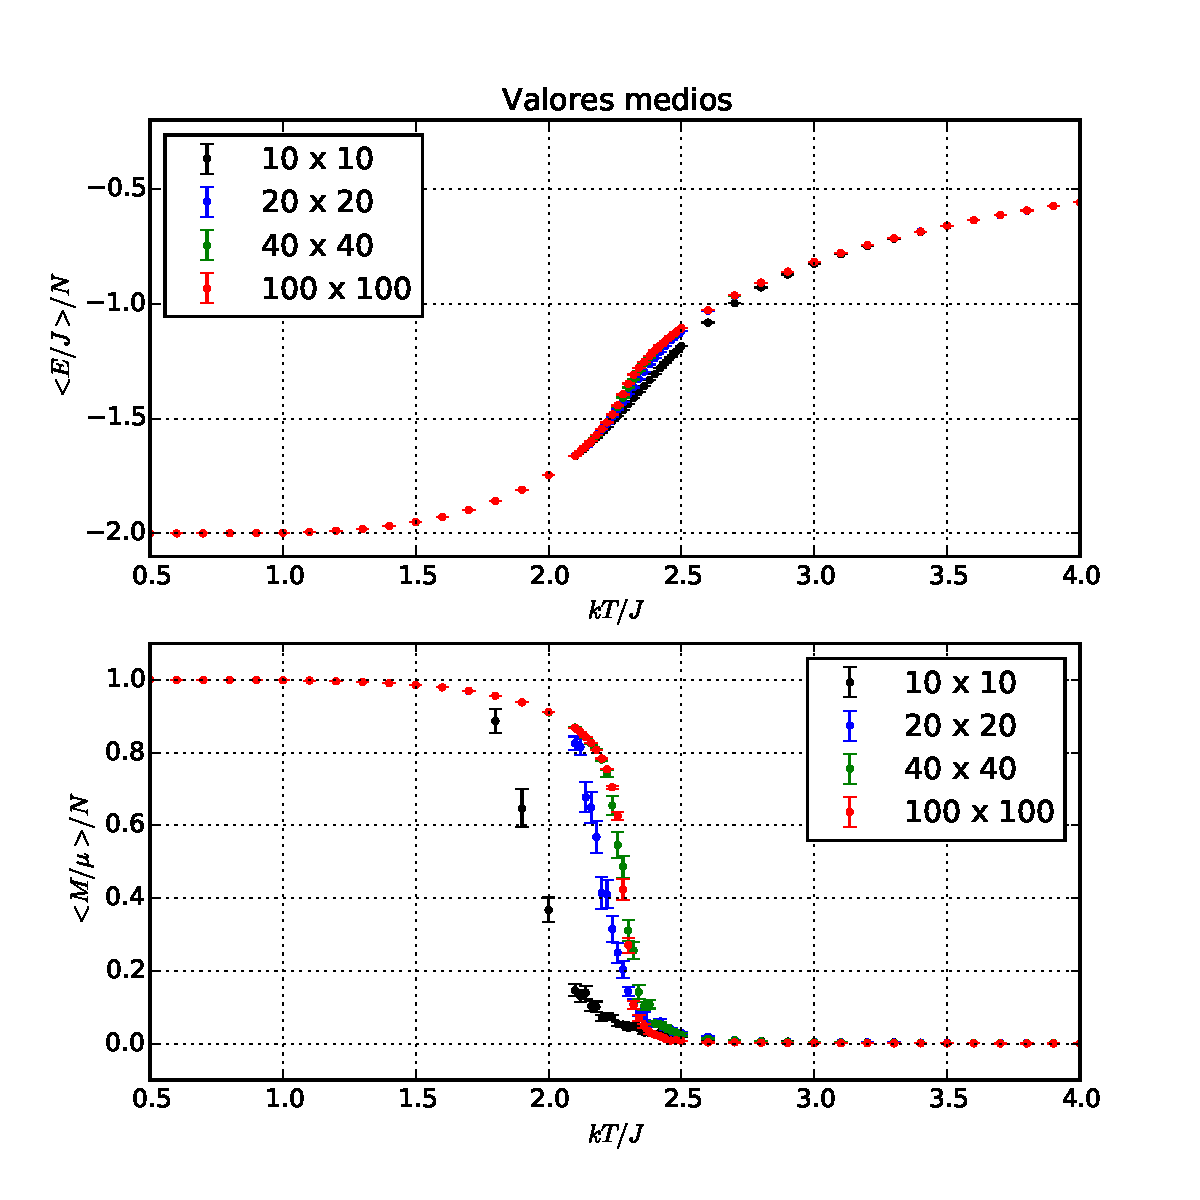
\includegraphics[scale=0.6]{tamano_val_medios.pdf} \\
      \caption{Distribuci�n poissonianas $P(4)$, $P(10)$ y $P(40)$. En rojo 
      aparecen las distribucciones gaussianas para cada 
      caso.}\label{fig:tam_val_medios}
    \end{center}
\end{figure}

\begin{figure}[H]
    \begin{center}
      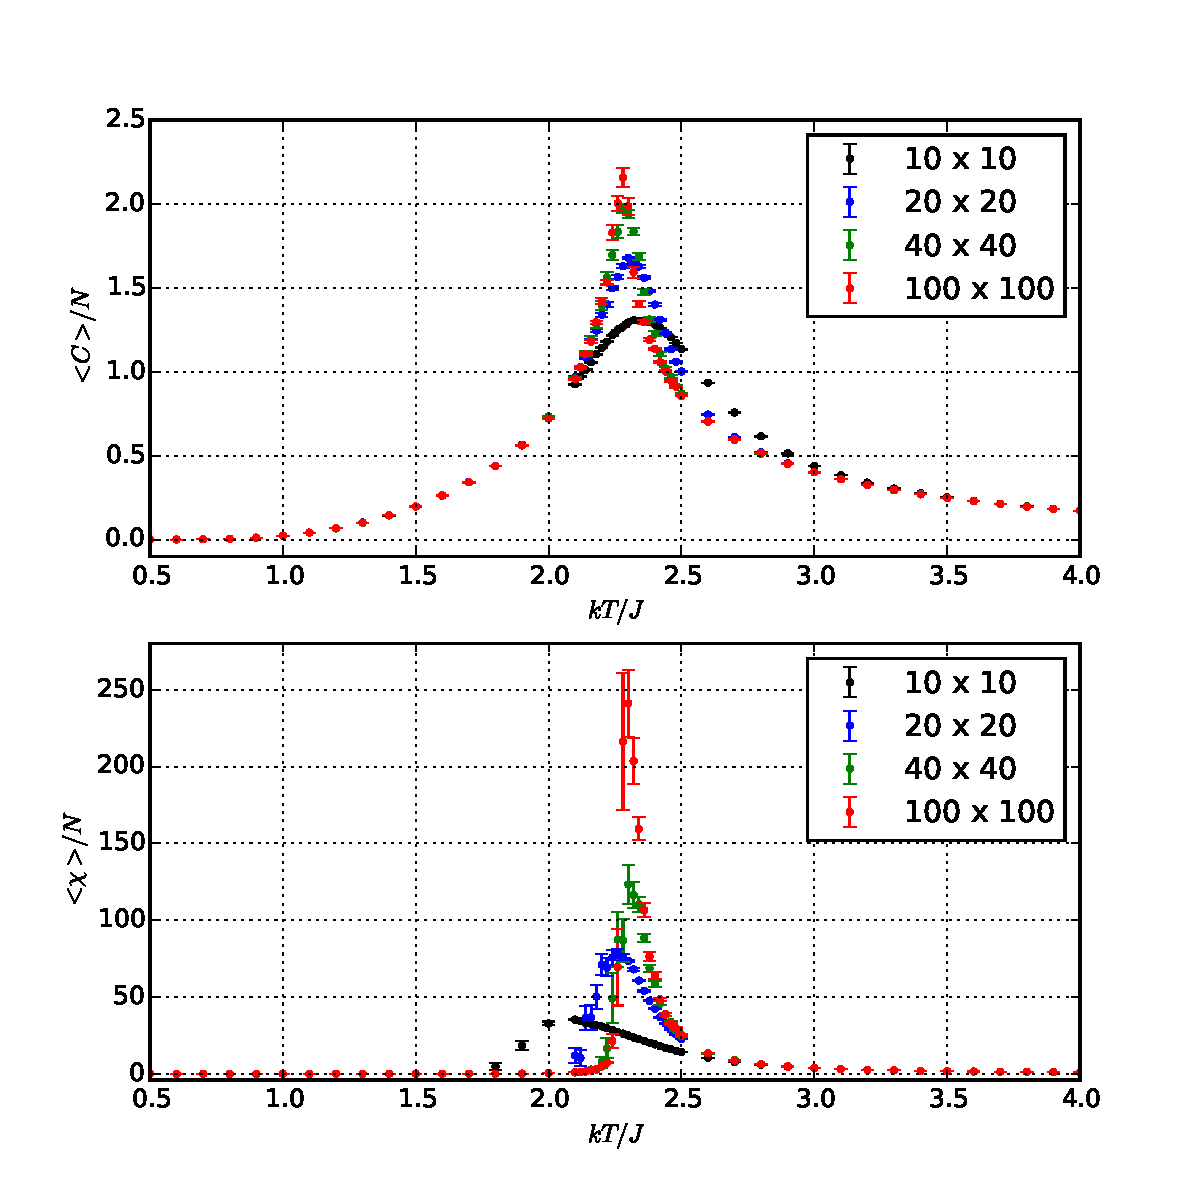
\includegraphics[scale=0.6]{tamano_fluctuaciones.pdf} \\
      \caption{Distribuci�n poissonianas $P(4)$, $P(10)$ y $P(40)$. En rojo 
      aparecen las distribucciones gaussianas para cada 
      caso.}\label{fig:fluctuaciones}
    \end{center}
\end{figure}

\begin{figure}[H]
    \begin{center}
      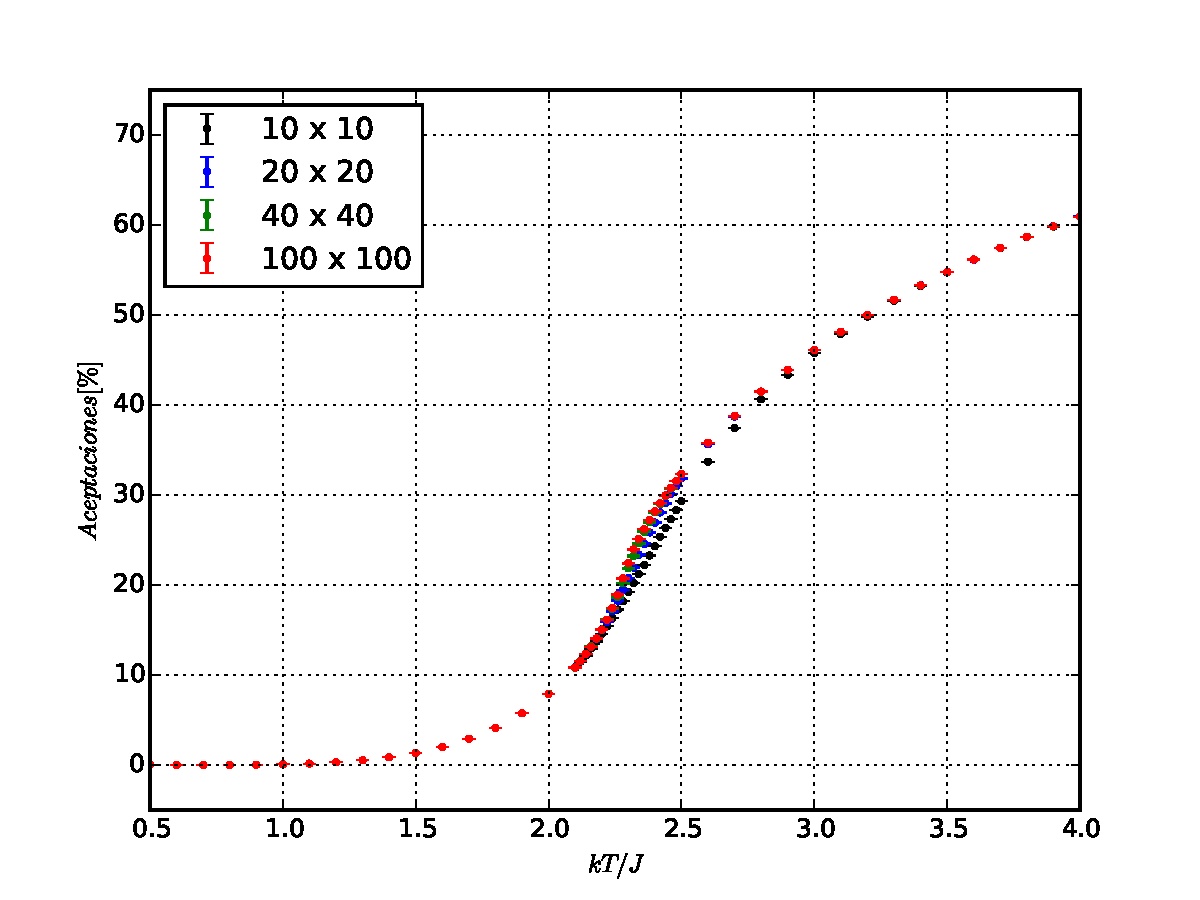
\includegraphics[scale=0.5]{tamano_aceptaciones.pdf} \\
      \caption{Distribuci�n poissonianas $P(4)$, $P(10)$ y $P(40)$. En rojo 
      aparecen las distribucciones gaussianas para cada 
      caso.}\label{fig:aceptaciones}
    \end{center}
\end{figure}

\begin{figure}[H]
    \begin{center}
      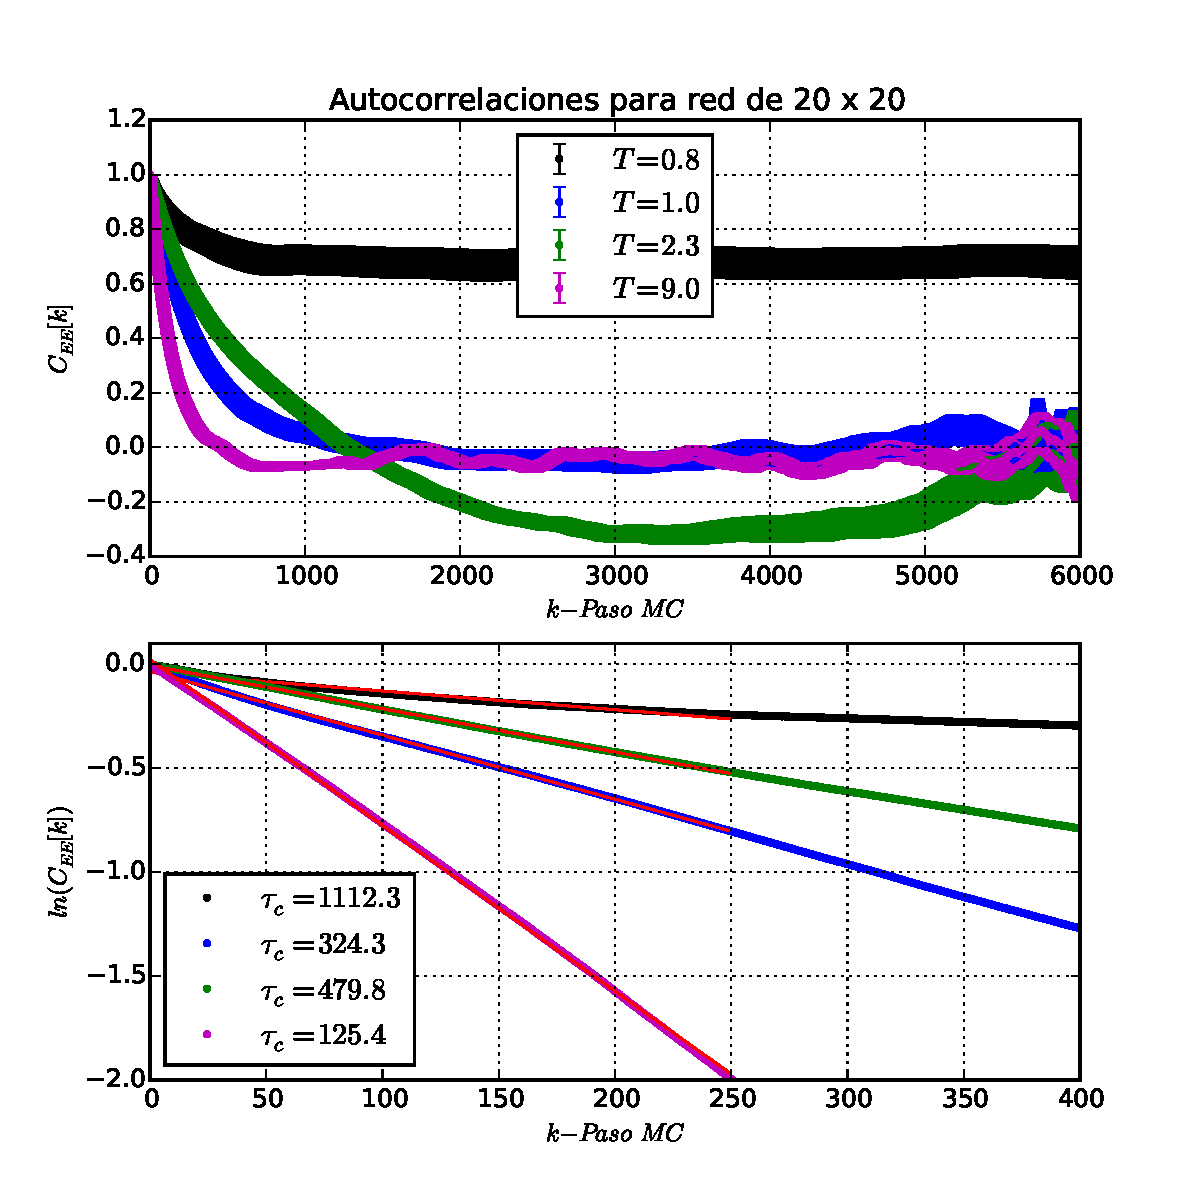
\includegraphics[scale=0.5]{corre_20x20.pdf} \\
      \caption{Distribuci�n poissonianas $P(4)$, $P(10)$ y $P(40)$. En rojo 
      aparecen las distribucciones gaussianas para cada 
      caso.}\label{fig:corre_20x20}
    \end{center}
\end{figure}

\begin{figure}[H]
    \begin{center}
      \includegraphics[scale=0.5]{{corre_tamano_t2.3}.pdf} \\
      \caption{Distribuci�n poissonianas $P(4)$, $P(10)$ y $P(40)$. En rojo 
      aparecen las distribucciones gaussianas para cada 
      caso.}\label{fig:corre_tamano_t2}
    \end{center}
\end{figure}

\begin{figure}[H]
    \begin{center}
      \includegraphics[scale=0.5]{{corre_tamano_t9.0}.pdf} \\
      \caption{Distribuci�n poissonianas $P(4)$, $P(10)$ y $P(40)$. En rojo 
      aparecen las distribucciones gaussianas para cada 
      caso.}\label{fig:corre_tamano_t9}
    \end{center}
\end{figure}

\end{document}
